% This tex file is available under a
% Creative Commons Attribution-Share Alike license (CC BY-SA 2.0).
% http://creativecommons.org/licenses/by-sa/2.0/
% Copyright © 2013 Rodrigo Hausen
\documentclass{beamer}
\usepackage[utf8]{inputenc}
\usepackage{lmodern}
\usepackage[T1]{fontenc}
\usepackage[portuguese,brazil]{babel}
\usepackage{url}
\usepackage{listings}
\usepackage{color}
\usepackage{textcomp}
\usepackage{pdfpages}
\usepackage{fancyvrb}
\usepackage{enumerate}
\usepackage{alltt}
\usepackage{array}
\usepackage{slashbox}
%\usepackage[pdf]{pstricks}
%\usepackage{auto-pst-pdf}
%\usepackage{icomma} % para vírgula decimal / decimal comma
\definecolor{listinggray}{gray}{0.9}
\definecolor{mediumgray}{rgb}{0.6,0.6,0.6}
\definecolor{lbcolor}{rgb}{0.9,0.9,0.9}
\lstset{
    backgroundcolor=\color{lbcolor},
    tabsize=4,
    rulecolor=,
    basicstyle=\scriptsize,
    upquote=true,
    aboveskip={1.5\baselineskip},
    columns=fixed,
    showstringspaces=false,
    extendedchars=true,
    breaklines=true,
    prebreak = \raisebox{0ex}[0ex][0ex]{\ensuremath{\hookleftarrow}},
    frame=single,
    showtabs=false,
    showspaces=false,
    showstringspaces=false,
    identifierstyle=\ttfamily,
    keywordstyle=\color[rgb]{0,0,1},
    commentstyle=\color[rgb]{0.133,0.545,0.133},
    stringstyle=\color[rgb]{0.627,0.126,0.941},
}
\definecolor{pinegreen}{RGB}{0,139,114}
\definecolor{pgr}{RGB}{0,139,114}

\definecolor{aquamarine}{RGB}{0,181,190}
\definecolor{aqm}{RGB}{0,181,190}

\definecolor{skyblue}{RGB}{100,227,251}
\definecolor{skb}{RGB}{100,227,251}

\definecolor{pnk}{RGB}{255,150,150}

\newcommand{\comment}[1]{{\color{structure.fg!70!white}\footnotesize #1}}

\newcommand{\WD}[1]{\fbox{#1}\hspace{-0.5pt}}
\newcommand{\FWD}[1]{%
\fbox{%
\vbox to 10pt{\vfil%
\hbox to 0.8cm{\hfill#1\hfill}%
\vfil}%
}\hspace{-0.5pt}%
}

\def\A{\texttt{A}}
\def\B{\texttt{B}}
\def\C{\texttt{C}}
\def\D{\texttt{D}}
\def\E{\texttt{E}}
\def\F{\texttt{F}}

\usetheme{Boadilla}
%\usetheme{umbc2}
\usefonttheme{structuresmallcapsserif}
\usecolortheme{seahorse}

\title{Aula 10: Blocos Digitais Básicos (Somador, Subtrator)}
\subtitle{Circuitos Digitais}
\author{Rodrigo Hausen}
\institute{CMCC -- UFABC} 
\date{25 de fevereiro de 2013}

\newcommand{\Not}[1]{\overline{#1}}
\def\And{\,}

\begin{document}

\begin{frame}
\maketitle

\vspace{-1cm}

\begin{center}
\url{http://compscinet.org/circuitos}
\end{center}

\end{frame}

%%%%%%%%%%%%%%%%%%%%%%%%%%%%%%%%%%%%%%%%%%%%%%%%%

\begin{frame}
\frametitle{Trabalho de casa:}

\begin{itemize}
\item Determine a expressão lógica mais simples para a saída de cada um dos
circuitos abaixo (os circuitos usam apenas portas \textbf{nand})
\end{itemize}
\begin{center}
\begin{minipage}{0.2\textwidth}
\only<1>{
\includegraphics[scale=0.9]{images/nand_univ1}}%
\only<2>{\includegraphics[scale=0.9]{images/nand_univ1_resp}}\\
Circuito 1
\end{minipage}
\hspace{8ex}
\begin{minipage}{0.4\textwidth}
\only<1>{\includegraphics[scale=0.9]{images/nand_univ2}}%
\only<2>{
\includegraphics[scale=0.9]{images/nand_univ2_resp}}\\
Circuito 2
\end{minipage}

\vspace{12pt}

\only<1>{
\includegraphics[scale=0.9]{images/nand_univ3}}%
\only<2>{\includegraphics[scale=0.9]{images/nand_univ3_resp}}\\
Circuito 3
\end{center}
\begin{itemize}
\item O que você pode concluir deste exercício?
\end{itemize}
 
\end{frame}

%%%%%%%%%%%%%%%%%%%%%%%%%%%%%%%%%%%%%%%%%%%%%%%%%
\begin{frame}
\frametitle{Universalidade da porta NAND}

Pense nisto:
\begin{enumerate}
\item Com as portas lógicas NOT, AND e OR, podemos calcular
\textbf{qualquer} função lógica;
\pause
\item Podemos construir as portas NOT, AND e OR usando apenas
portas NAND:
\begin{center}
\begin{minipage}{0.2\textwidth}
\includegraphics[scale=0.9]{images/nand_univ1_resp}
\end{minipage}
\hspace{8ex}
\begin{minipage}{0.4\textwidth}

\includegraphics[scale=0.9]{images/nand_univ2_resp}
\end{minipage}

\vspace{12pt}

\includegraphics[scale=0.9]{images/nand_univ3_resp}
\end{center}
\end{enumerate}

\pause

\textbf{Conclusão:} posso construir qualquer circuito digital
usando apenas portas NAND.
\end{frame}

%%%%%%%%%%%%%%%%%%%%%%%%%%%%%%%%%%%%%%%%%%%%%%%%%
\begin{frame}
\frametitle{Universalidade da porta NOR}

\begin{itemize}
\item \textbf{Para casa: } mostre que podemos construir \textbf{qualquer}
circuito digital usando apenas portas NOR.
\end{itemize}

\end{frame}

%%%%%%%%%%%%%%%%%%%%%%%%%%%%%%%%%%%%%%%%%%%%%%%%%
\begin{frame}
\frametitle{Blocos Digitais Básicos}

\begin{minipage}{0.7\textwidth}
\begin{itemize}
\item Os blocos mais elementares da eletrônica digital são as
portas lógicas.
\end{itemize}
\end{minipage}
\begin{minipage}{0.27\textwidth}
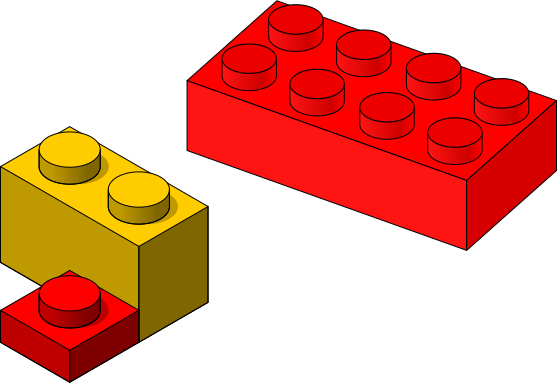
\includegraphics[width=0.9\textwidth]{images/bricks}
% Fontes:
% http://en.wikipedia.org/wiki/File:Plastic_brick,_red.svg
% http://upload.wikimedia.org/wikipedia/commons/archive/1/1a/20110410000706%21Lego_dimensions.svg
\end{minipage}
\pause
\begin{itemize}
\item Daqui em diante, vamos aplicar o nosso conhecimento de
análise e síntese de circuitos digitais para construir alguns
blocos um pouco menos elementares:
\pause
\begin{itemize}
\item somadores e subtratores
\pause
\item codificadores e decodificadores
\pause
\item multiplexadores e demultiplexadores
\pause
\item unidades lógico-aritméticas
\pause
\item latches e flip-flops
\pause
\item registradores e memórias
\end{itemize}
\pause
\item É extremamente útil saber a função de cada um desses blocos
e as suas interfaces (ou seja, como conectar cada um deles em
nossos circuitos).
\end{itemize}
\end{frame}

%%%%%%%%%%%%%%%%%%%%%%%%%%%%%%%%%%%%%%%%%%%%%%%%%

\begin{frame}
\frametitle{Blocos somadores binários}

\begin{itemize}
\item \textbf{Exemplo 1}: Elabore um circuito digital com $2$ entradas, $a_0$ e $b_0$, e $2$ saídas, $s_1$ e $s_0$ de tal forma que $(s_1 s_0)_2$ represente a soma aritmética $a_0 + b_0$.
\vspace{-12pt}
\begin{center}
\begin{tabular}{cc@{}c@{\,}c}
  && & $a_0$ \\
+ && & $b_0$ \\
\cline{2-4}
  && $s_1$ & $s_0$
\end{tabular}
\end{center}

\pause

\item \textbf{Primeiro passo}: obtenha e simplifique a expressão lógica
para cada saída.

\pause

\begin{center}
\begin{tabular}{cc||c}
$a_0$ & $b_0$ & $s_0$ \\
\hline
  0   &   0   &   0   \\
  0   &   1   &   1   \\
  1   &   0   &   1   \\
  1   &   1   &   0
\end{tabular}
\hspace{6ex}
\begin{tabular}{cc||c}
$a_0$ & $b_0$ & $s_1$ \\
\hline
  0   &   0   &   0   \\
  0   &   1   &   0   \\
  1   &   0   &   0   \\
  1   &   1   &   1
\end{tabular}
\end{center}

\pause

\item Neste caso, é elementar obter expressões simples para as saídas:\\
$s_0 = a_0 \oplus b_0$\\
$s_1 = a_0 b_0$

\end{itemize}


\end{frame}


%%%%%%%%%%%%%%%%%%%%%%%%%%%%%%%%%%%%%%%%%%%%%%%%%

\begin{frame}
\frametitle{Blocos somadores binários}

\begin{itemize}
\item \textbf{Exemplo 1}: Elabore um circuito digital com $2$ entradas, $a_0$ e $b_0$, e $2$ saídas, $s_1$ e $s_0$ de tal forma que $(s_1 s_0)_2$ represente a soma aritmética $a_0 + b_0$.

\item \textbf{Segundo passo}: desenhar o diagrama do circuito.\\
$s_0 = a_0 \oplus b_0$ \; e \; $s_1 = a_0 b_0$ (note que há um \textbf{and} implícito)\\[6pt]

\begin{center}
\only<1>{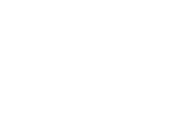
\includegraphics{images/exemplo4_0}}%
\only<2>{\includegraphics{images/exemplo4_1}}%
\only<3>{
\includegraphics{images/exemplo4_2}}%
\only<4>{\includegraphics{images/exemplo4_3}}%
\only<5->{\includegraphics{images/exemplo4}}
\end{center}

\pause\pause\pause\pause\pause

\item \textbf{Terceiro passo}: analisar o circuito e verificar as saídas.

\pause

\item \textbf{Quarto passo}: monte o circuito e faça sua tabela verdade.\\
\comment{(para este circuito, os dois últimos passos não tem a menor graça)} 

\end{itemize}
\end{frame}

%%%%%%%%%%%%%%%%%%%%%%%%%%%%%%%%%%%%%%%%%%%%%%%%%

\newcommand{\INP}[1]{\fcolorbox{white}{pnk}{#1}}
\newcommand{\OUT}[1]{\fcolorbox{white}{skb}{#1}}

\begin{frame}
\frametitle{Blocos somadores binários}

\begin{itemize}
\item \textbf{Exemplo 2}: Elabore um circuito digital com $3$ entradas, $a_i$, $b_i$, $c_{i-1}$ e $2$ saídas, $s_i$ e $c_i$ de tal forma que $s_i$ represente a soma aritmética $a_i + b_i + c_{i-1}$ e $c_i$ represente o vai-um (carry) da operação.

\end{itemize}

\begin{center}
\begin{tabular}{rc@{}c@{\,}c@{\,}c@{\,}c@{\,}c@{\,}c}
vai-uns $\rightarrow$
 & & $c_{i+1}$ & \OUT{$c_{i}$} & \INP{$c_{i-1}$}           & \ldots & $c_0$ &       \\
 & & \ldots    & $a_{i+1}$     & \INP{$a_{i\phantom{-1}}$} & \ldots & $a_1$ & $a_0$ \\
+& & \ldots    & $b_{i+1}$     & \INP{$b_{i\phantom{-1}}$} & \ldots & $b_1$ & $b_0$ \\
\cline{2-8}
 & & \ldots    & $s_{i+1}$     & \OUT{$s_{i\phantom{-1}}$} & \ldots & $s_1$ & $s_0$
\end{tabular}
\end{center}

\pause

\begin{itemize}
\item Quais são as entradas? \pause $a_i$, $b_i$, $c_{i-1}$ \pause
\item Quais são as saídas? \pause $s_i$, $c_i$
\end{itemize}

\end{frame}

%%%%%%%%%%%%%%%%%%%%%%%%%%%%%%%%%%%%%%%%%%%%%%%%%
\begin{frame}
\frametitle{Blocos somadores binários}

\begin{itemize}
\item \textbf{Primeiro passo}: obter as expressões para as saídas $s_i$ e $c_i$. 
\end{itemize}

\begin{center}
\begin{tabular}{rc@{}c@{\,}c@{\,}c@{\,}c@{\,}c@{\,}c}
vai-uns $\rightarrow$
 & & $c_{i+1}$ & \OUT{$c_{i}$} & \INP{$c_{i-1}$}           & \ldots & $c_0$ &       \\
 & & \ldots    & $a_{i+1}$     & \INP{$a_{i\phantom{-1}}$} & \ldots & $a_1$ & $a_0$ \\
+& & \ldots    & $b_{i+1}$     & \INP{$b_{i\phantom{-1}}$} & \ldots & $b_1$ & $b_0$ \\
\cline{2-8}
 & & \ldots    & $s_{i+1}$     & \OUT{$s_{i\phantom{-1}}$} & \ldots & $s_1$ & $s_0$
\end{tabular}
\end{center}

\pause

\begin{minipage}{0.49\textwidth}

Para a soma $s_i$:

\begin{tabular}{|c|c|c|c|c|}
\hline
\backslashbox{$c_{i-1}$\hspace*{-3ex}}{\hspace*{-4ex}$a_i b_i$}
   & 00 & 01 & 11 & 10 \\
\hline
 0 &  0 &  1 &  0 &  1 \\
\hline
 1 &  1 &  0 &  1 &  0 \\
\hline
\end{tabular}

\end{minipage}
%
\pause
%
\begin{minipage}{0.49\textwidth}

Para o vai-um $c_i$:

\begin{tabular}{|c|c|c|c|c|}
\hline
\backslashbox{$c_{i-1}$\hspace*{-3ex}}{\hspace*{-4ex}$a_i b_i$}
   & 00 & 01 & 11 & 10 \\
\hline
 0 &  0 &  0 &  1 &  0 \\
\hline
 1 &  0 &  1 &  1 &  1 \\
\hline
\end{tabular}

\end{minipage}

\end{frame}

%%%%%%%%%%%%%%%%%%%%%%%%%%%%%%%%%%%%%%%%%%%%%%%%%

\begin{frame}
\frametitle{Blocos somadores binários}

\begin{itemize}
\item \textbf{Primeiro passo}: (continuação)
\end{itemize}

\vspace{6pt}

\hspace{0.05\textwidth}
\begin{minipage}{0.45\textwidth}

Para a soma $s_i$:

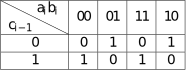
\includegraphics{images/exemplo5_tabela_si}

\end{minipage}
%
\begin{minipage}{0.4\textwidth}

Para o vai-um $c_i$:

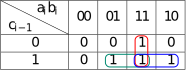
\includegraphics{images/exemplo5_tabela_ci}

\end{minipage}

\vspace{12pt}

\pause

Note que $s_i$ só é $1$ se apenas um dos bits $a_i$, $b_i$, $c_{i-1}$ é
$1$, ou se os três forem $1$. Isto corresponde à expressão:\\
$s_i = a_i \oplus b_i \oplus c_{i-1}$

\vspace{12pt}

\pause

$c_i = {\color{red}a_i b_i} + {\color{blue}a_i c_{i-1}} + {\color{pgr} b_i c_{i-1}} \pause = a_i b_i + (a_i + b_i ) \cdot c_{i-1}$

\end{frame}

%%%%%%%%%%%%%%%%%%%%%%%%%%%%%%%%%%%%%%%%%%%%%%%%%

\begin{frame}
\frametitle{Blocos somadores binários}

\begin{itemize}

\item \textbf{Segundo passo}: diagrama do circuito digital.

\end{itemize}

\begin{minipage}{0.47\textwidth}
\hspace{4ex} $s_i = a_i \oplus b_i \oplus c_{i-1}$
\end{minipage}
%
\begin{minipage}{0.47\textwidth}
$c_i = a_i b_i + (a_i + b_i ) \cdot c_{i-1}$
\end{minipage}

\begin{center}
\only<1>{\includegraphics{images/exemplo5_0}}%
\only<2>{\includegraphics{images/exemplo5_1}}%
\only<3>{\includegraphics{images/exemplo5_2}}%
\only<4>{\includegraphics{images/exemplo5_3}}%
\only<5>{\includegraphics{images/exemplo5_4}}%
\only<6>{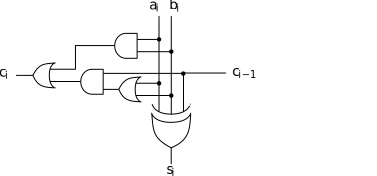
\includegraphics{images/exemplo5_5}}%
\only<7->{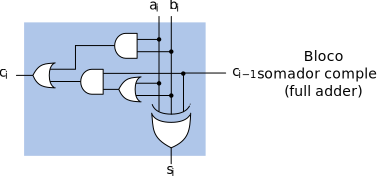
\includegraphics{images/exemplo5}}%
\end{center}

\pause\pause\pause\pause\pause\pause\pause

\comment{(Terceiro passo foi feito na aula passada. Vamos omitir
o quarto passo.)}

\end{frame}

%%%%%%%%%%%%%%%%%%%%%%%%%%%%%%%%%%%%%%%%%%%%%%%%%

\begin{frame}
\frametitle{Blocos somadores binários}

\begin{itemize}
\item Note que, juntando blocos Half Adder e Full Adder, podemos montar um
somador para números de $n$ bits.
\end{itemize}

\begin{center}
{\small
\begin{tabular}{rc@{}c@{\,}c@{\,}c@{\,}c@{\,}c@{\,}c}
 & & \OUT{$c_{n-1}$} & $c_{n-2}$ & $c_{n-3}$       & \ldots & $c_0$ &       \\
 & &                 & \INP{$a_{n-1}$} & \INP{$a_{n-2}$} & \ldots & \INP{$a_1$} & \INP{$a_0$} \\
+& &                 & \INP{$b_{n-1}$} & \INP{$b_{n-2}$} & \ldots & \INP{$b_1$} & \INP{$b_0$} \\
\cline{2-8}
 & &                 & \OUT{$s_{n-1}$} & \OUT{$s_{n-2}$} & \ldots & \OUT{$s_1$} & \OUT{$s_0$}
\end{tabular}}

\vspace{6pt}

\only<1>{\includegraphics{images/somador_0}}%
\only<2>{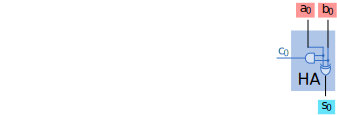
\includegraphics{images/somador_1}}%
\only<3>{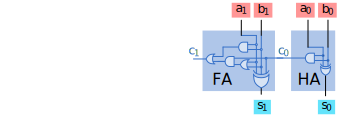
\includegraphics{images/somador_2}}%
\only<4>{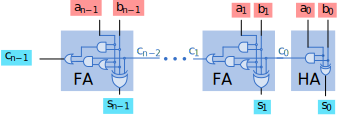
\includegraphics{images/somador}}%
\end{center}

\end{frame}


%%%%%%%%%%%%%%%%%%%%%%%%%%%%%%%%%%%%%%%%%%%%%%%%%

\begin{frame}
\frametitle{Blocos somadores binários}

\begin{itemize}
\item \textbf{Somador ripple carry de $n$ bits}: leva este nome pois os
vai-uns (carry) são propagados como uma ondulação (ripple) da direita para
a esquerda.
\end{itemize}

\begin{center}
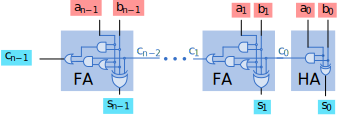
\includegraphics{images/somador}
\end{center}

\begin{itemize}
\item \textbf{Para casa}: diga quantas e quais são as portas lógicas usadas
(separe as portas lógicas com $2$ entradas das de $3$ entradas) em um
somador ripple carry de $n$ bits.
\end{itemize}

\end{frame}

%%%%%%%%%%%%%%%%%%%%%%%%%%%%%%%%%%%%%%%%%%%%%%%%%

\begin{frame}
\frametitle{Blocos somadores binários}

\begin{itemize}
\item Podemos enxergar os blocos somadores (half adder e full adder)
como caixas-pretas.\\
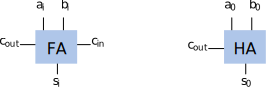
\includegraphics{images/ripple_carry}
\pause
\item Também podemos enxergar um somador de $n$ bits como uma
caixa-preta:
\end{itemize}
\begin{minipage}{60mm}
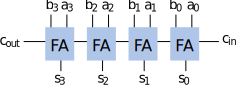
\includegraphics[width=60mm]{images/fulladder_4bits}
\end{minipage}
\hfill
{\Huge =}
\hfill
\begin{minipage}{39mm}
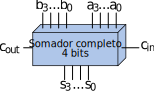
\includegraphics[width=39mm]{images/fulladder_4bits_blackbox}
\end{minipage}

\end{frame}

%%%%%%%%%%%%%%%%%%%%%%%%%%%%%%%%%%%%%%%%%%%%%%%%%

\begin{frame}
\frametitle{Blocos somadores binários}

\begin{itemize}
\item Podemos comprar blocos somadores integrados: 7483 (TTL); CD4008 (CMOS); e outros.\\
\hspace*{\fill}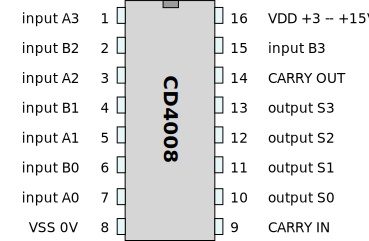
\includegraphics[height=25ex]{images/4008}\hspace*{\fill}
% Source: http://www.doctronics.co.uk/4008.htm
\pause
\item Podemos unir blocos somadores completos para obter somadores com
quantidade maior de bits (p. ex. juntar 8 integrados CD4008 para fazer
um somador de 32 bits)
\end{itemize}
\end{frame}

%%%%%%%%%%%%%%%%%%%%%%%%%%%%%%%%%%%%%%%%%%%%%%%%%

\begin{frame}
\frametitle{Bloco subtrator binário}

\begin{itemize}
\item E a subtração?
\pause
\item Lembra da subtração feita usando-se complemento a $2$?\\
$B = (b_{n-1} \; b_{n-2} \; \ldots \; b_{1} \; b_{0})_2$\\[3pt]
$A = (a_{n-1} \; a_{n-2} \; \ldots \; a_{1} \; a_{0})_2$\\[6pt]
\pause
$\overline{A} = (\overline{a_{n-1}} \; \overline{a_{n-2}} \; \ldots \; \overline{a_{1}} \; \overline{a_{0}})_2$ (complemento a um de $A$)\\[6pt]
\pause
$B - A \; \; = \; \; B + \underbrace{\overline{A} + 1}_{\!\!\!\!\text{compl. a $2$}\!\!\!\!}$ e despreza-se o último vai-um
\pause
\item Faça o diagrama de um circuito digital para um subtrator de $n$ bits.
Você só precisará de:
\begin{itemize}
\item um somador completo de $n$ bits; e
\item portas NOT
\end{itemize}
(resposta na lousa)
\end{itemize}
\end{frame}

%%%%%%%%%%%%%%%%%%%%%%%%%%%%%%%%%%%%%%%%%%%%%%%%%

\begin{frame}
\frametitle{Soma e subtração de números com sinal}

\begin{itemize}
\item Este é um somador para palavras de $n$ bits que representam
números inteiros sem sinal.\\
{\centering%
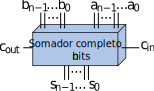
\includegraphics{images/fulladder_Nbits_blackbox}\\}
\item Como é um somador para palavras de $n$ bits que representam
números inteiros com sinal no formato complemento de $2$?\\[8pt]
\pause
{\centering%
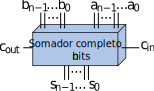
\includegraphics{images/fulladder_Nbits_blackbox}\\}
\pause
\item Não há nenhuma diferença no circuito!
\end{itemize}

\end{frame}

%%%%%%%%%%%%%%%%%%%%%%%%%%%%%%%%%%%%%%%%%%%%%%%%%

\begin{frame}
\frametitle{Soma e subtração de números com sinal}

\begin{itemize}
\item Em casa, monte um somador binário para números
de 5 bits no Logisim, usando 5 somadores completos
de 1 bit. Faça as somas abaixo usando a representação
de complemento de $2$ (manualmente e no Logisim) e
interprete os resultados:
\end{itemize}

\begin{center}
\begin{tabular}{l@{\hspace{8ex}}l}
a) (+3) + (+6)   &    b) (+6) + (+3) \\[12pt]
c) (-3) + (+6)   &    d) (+6) + (-3) \\[12pt]
e) (-3) + (-6)   &    f) (+7) + (+9) \\[12pt]
g) (-7) + (-9)   &    h) (-8) + (-9)
\end{tabular}
\end{center}
\end{frame}

%%%%%%%%%%%%%%%%%%%%%%%%%%%%%%%%%%%%%%%%%%%%%%%%%

\begin{frame}
\frametitle{Comparação entre números}

\textbf{Exercício 1}: Seja $X = x_{n-1} x_{n-2} \ldots x_1 x_0$ uma palavra
de $n$ bits que representa um número inteiro com sinal no formato de complemento
de $2$. Faça um circuito digital com $n$ entradas e $3$ saídas:
\begin{itemize}
\item $f_{X<0}$, que é $1$ se $X$ representa um número negativo, $0$
caso contrário
\item $f_{X=0}$, que é $1$ se $X$ representa o número zero, $0$
caso contrário
\item $f_{X>0}$, que é $1$ se $X$ representa um número positivo, $0$
caso contrário
\end{itemize}

\pause

\vspace{12pt}

\textbf{Exercício 2}: Faça um circuito digital com $2n$ entradas e $3$ saídas
$f_{B<A}$, $f_{B>A}$ e $f_{B=A}$ que são $1$, respectivamente, se
$B<A$ ou $B>A$ ou $B=A$, onde $A$, $B$ são palavras de $n$ que representam
números inteiros com sinal no formato de complemento de $2$.
\pause
\begin{itemize}
\item Dica: qual é o sinal de $B - A$?
\pause
$$
B - A \text{ é } \left\{
\begin{array}{l}
\text{\textbf{negativo} se, e somente se, } B < A \\ \pause
= 0 \text{ se, e somente se, } B = A \\ \pause
\text{\textbf{positivo} se, e somente se, } B > A
\end{array}
\right.
$$
\end{itemize}
\pause
\comment{(respostas na lousa)}

\end{frame}

%%%%%%%%%%%%%%%%%%%%%%%%%%%%%%%%%%%%%%%%%%%%%%%%%

\begin{frame}
\frametitle{Para casa}

\begin{itemize}
\item Leia a seção 5-3 e faça os seguintes exercícios do capítulo 5:\\
autotestes 7 a 10; problemas 18 a 21.
\item Leia as seções 6-1, 6-2, 6-4 (o Floyd faz comparação de números
de maneira diferente) e faça os seguintes exercícios do capítulo 6:\\
autotestes 1 a 6; problemas 1 a 7, 11 a 13.
\item Leia a seção 6-3 apenas para aumentar sua cultura.
\end{itemize}
\end{frame}

%%%%%%%%%%%%%%%%%%%%%%%%%%%%%%%%%%%%%%%%%%%%%%%%%

\begin{frame}
\frametitle{Para casa}

\begin{itemize}
\item \textbf{Problema 1:} Faça um circuito para detectar overflow
em uma operação de (a) soma e (b) subtração entre duas palavras de
$n$ bits que representam inteiros com sinal no formato complemento
de $2$\\[12pt]
\pause
\item \textbf{Problema 2:} Sem usar blocos somadores/subtratores,
faça um circuito digital
para calcular o produto de dois números inteiros sem sinal com dois
bits cada um. Esse circuito terá \only<2>{\phantom{4}}\only<3->{4} entradas
e \only<2>{\phantom{4}}\only<3->{4} saídas.
\end{itemize}

\pause
\begin{center}
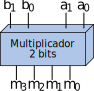
\includegraphics{images/multiplier}
\end{center}
\end{frame}

%%%%%%%%%%%%%%%%%%%%%%%%%%%%%%%%%%%%%%%%%%%%%%%%%

\begin{frame}
\frametitle{Para casa}

\begin{itemize}
\item \textbf{Problema 3:} Faça um circuito com $n+1$ entradas,
$x_{n-1}, x_{n-2}, \ldots, x_1, x_0, y$ e $n$ saídas
$z_{n-1}, z_{n-1}, \ldots, z_1, z_0$ tal que:
$$
\text{para todo } i \text{ entre } 0 \text{ e } n-1 \text{, }
z_i = \left\{
 \begin{array}{l}
   0 \text{ se } y = 0 \\
   x_i \text{ se } y = 1
 \end{array} \right.
$$
(resolva primeiro para $1$, $2$, $3$, \ldots)
\end{itemize}

\pause

\begin{center}
\only<1-2,5>{\includegraphics{images/selector}}%
\only<3>{\includegraphics{images/selector0}}%
\only<4>{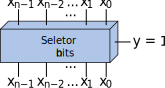
\includegraphics{images/selector1}}%
\end{center}

\end{frame}

%%%%%%%%%%%%%%%%%%%%%%%%%%%%%%%%%%%%%%%%%%%%%%%%%

\begin{frame}
\frametitle{Para casa}

\begin{itemize}
\item \textbf{Problema 4:} Faça um multiplicador para dois números
sem sinal de dois bits cada, agora usando blocos somadores.\\[12pt]
\pause
\item \textbf{Problema 5:} Idem 4, mas agora para números de $n$ bits
sem sinal
\comment{(pode ajudar se você pensar nos casos particulares primeiro:
$n=3$, $n=4$, \ldots)}
\end{itemize}
\end{frame}

%%%%%%%%%%%%%%%%%%%%%%%%%%%%%%%%%%%%%%%%%%%%%%%%%

\begin{frame}
\frametitle{Projeto de final de semana}

\textbf{Decodificador de controle remoto}: com este circuito simples,
você poderá ver a forma de onda emitida por um controle remoto de
TV/DVD/aparelho de som/etc. Você irá gastar em torno de $6$ reais nestas
peças:
\begin{itemize}
\item $1$ fototransistor infravermelho (receptor infravermelho);
\item $1$ cabo de áudio com um plug P2 macho em uma ponta e dois
ou três plugs RCA macho na outra (cabo para ligar o computador em amplificador).
\end{itemize}

\begin{minipage}{20ex}%
\includegraphics[width=20ex]{images/fototransistor}%
\end{minipage}%
\hfill e \hfill%
\begin{minipage}{18ex}%
\includegraphics[width=20ex]{images/cabop2rcap2}%
\end{minipage}%
\hfill ou \hfill%
\begin{minipage}{20ex}%
\includegraphics[width=20ex]{images/cabo_filmadora}%
\end{minipage}%

\end{frame}

%%%%%%%%%%%%%%%%%%%%%%%%%%%%%%%%%%%%%%%%%%%%%%%%%

\begin{frame}
\frametitle{Projeto de final de semana}

{\small
\begin{enumerate}
\item Primeiro, veja quantas conexões de áudio o seu computador tem:
\begin{itemize}
\item Se o seu computador possui pelo menos duas conexões
para áudio (uma para fone de ouvido/caixa de som, e outra para
microfone) compre o cabo com $2$ plugs RCA.
\item Se seu computador só possui uma conexão para áudio,
compre o cabo com $3$ plugs RCA
\end{itemize}
\pause
\item Vá em uma loja de eletrônica e compre os materiais.
\pause
\item Baixe e execute o Audacity: \url{http://audacity.sourceforge.net}
\pause
\item Plugue o cabo na entrada de microfone do seu computador.
\pause
\item Com sua mão, mantenha o terminal mais comprido do fototransistor
ligado ao pino interno do plug RCA, e o terminal mais curto ligado à conexão
externa (se seu computador só possui 1 conexão de áudio, use o plug amarelo;
caso contrário, use o vermelho)
\pause
\item Pressione a tecla R no computador para gravar o ``áudio'' do microfone
\pause
\item Encoste o controle remoto no fototransistor e pressione qualquer
botão do controle
\end{enumerate}
}
\end{frame}

%%%%%%%%%%%%%%%%%%%%%%%%%%%%%%%%%%%%%%%%%%%%%%%%%

\begin{frame}
\frametitle{Projeto de final de semana}

\begin{itemize}
\item Resultado:
\end{itemize}
\includegraphics[width=\textwidth]{images/remote-dvd-lg-rh255-PLAY-wav-76000Hz}

\begin{itemize}
\item Resultados podem variar de acordo com a iluminação
ambiente, controle remoto, qualidade da placa de som do computador e
configuração dos astros.
\item Se esta experiência não funcionar para você, nem tudo está perdido:
\begin{itemize}
\item o cabo pode ser usado para ligar o áudio do seu computador na sua
TV ou aparelho de som!
\item é possível fazer um circuito um pouco mais sensível, que garantidamente
funcione, mas é necessário saber montar circuitos.
\end{itemize}
\end{itemize}

\end{frame}

%%%%%%%%%%%%%%%%%%%%%%%%%%%%%%%%%%%%%%%%%%%%%%%%%

\begin{frame}
\frametitle{Projeto de final de semana}

\begin{itemize}
\item Se você quer gastar menos, e tiver um fone de ouvido com defeito
(todo mundo tem um no fundo de alguma gaveta), dá para desencapar o
cabo do fone e usá-lo para conectar o fototransistor ao computador.
\begin{itemize}
\item se você já tiver o cabo, o custo fica em menos de 1 real!
\item mais informações:
\end{itemize}
\end{itemize}
{\small
\url{http://jumpjack.wordpress.com/2008/05/20/worlds-cheapest-remote-control-replicator-just-1/}}
\end{frame}

\end{document}
